% Options for packages loaded elsewhere
\PassOptionsToPackage{unicode}{hyperref}
\PassOptionsToPackage{hyphens}{url}
\PassOptionsToPackage{dvipsnames,svgnames,x11names}{xcolor}
%
\documentclass[journal=asbcd6,manuscript=article,layout=traditional]{achemso}
\usepackage[version=3]{mhchem}
\newcommand*\mycommand[1]{\texttt{\emph{#1}}}



\usepackage{amsmath,amssymb}
\usepackage{iftex}
\ifPDFTeX
  \usepackage[T1]{fontenc}
  \usepackage[utf8]{inputenc}
  \usepackage{textcomp} % provide euro and other symbols
\else % if luatex or xetex
  \usepackage{unicode-math}
  \defaultfontfeatures{Scale=MatchLowercase}
  \defaultfontfeatures[\rmfamily]{Ligatures=TeX,Scale=1}
\fi
\usepackage{lmodern}
\ifPDFTeX\else  
    % xetex/luatex font selection
\fi
% Use upquote if available, for straight quotes in verbatim environments
\IfFileExists{upquote.sty}{\usepackage{upquote}}{}
\IfFileExists{microtype.sty}{% use microtype if available
  \usepackage[]{microtype}
  \UseMicrotypeSet[protrusion]{basicmath} % disable protrusion for tt fonts
}{}
\makeatletter
\@ifundefined{KOMAClassName}{% if non-KOMA class
  \IfFileExists{parskip.sty}{%
    \usepackage{parskip}
  }{% else
    \setlength{\parindent}{0pt}
    \setlength{\parskip}{6pt plus 2pt minus 1pt}}
}{% if KOMA class
  \KOMAoptions{parskip=half}}
\makeatother
\usepackage{xcolor}
\setlength{\emergencystretch}{3em} % prevent overfull lines
\setcounter{secnumdepth}{-\maxdimen} % remove section numbering
% Make \paragraph and \subparagraph free-standing
\ifx\paragraph\undefined\else
  \let\oldparagraph\paragraph
  \renewcommand{\paragraph}[1]{\oldparagraph{#1}\mbox{}}
\fi
\ifx\subparagraph\undefined\else
  \let\oldsubparagraph\subparagraph
  \renewcommand{\subparagraph}[1]{\oldsubparagraph{#1}\mbox{}}
\fi


\providecommand{\tightlist}{%
  \setlength{\itemsep}{0pt}\setlength{\parskip}{0pt}}\usepackage{longtable,booktabs,array}
\usepackage{calc} % for calculating minipage widths
% Correct order of tables after \paragraph or \subparagraph
\usepackage{etoolbox}
\makeatletter
\patchcmd\longtable{\par}{\if@noskipsec\mbox{}\fi\par}{}{}
\makeatother
% Allow footnotes in longtable head/foot
\IfFileExists{footnotehyper.sty}{\usepackage{footnotehyper}}{\usepackage{footnote}}
\makesavenoteenv{longtable}
\usepackage{graphicx}
\makeatletter
\def\maxwidth{\ifdim\Gin@nat@width>\linewidth\linewidth\else\Gin@nat@width\fi}
\def\maxheight{\ifdim\Gin@nat@height>\textheight\textheight\else\Gin@nat@height\fi}
\makeatother
% Scale images if necessary, so that they will not overflow the page
% margins by default, and it is still possible to overwrite the defaults
% using explicit options in \includegraphics[width, height, ...]{}
\setkeys{Gin}{width=\maxwidth,height=\maxheight,keepaspectratio}
% Set default figure placement to htbp
\makeatletter
\def\fps@figure{htbp}
\makeatother

\makeatletter
\makeatother
\makeatletter
\makeatother
\makeatletter
\@ifpackageloaded{caption}{}{\usepackage{caption}}
\AtBeginDocument{%
\ifdefined\contentsname
  \renewcommand*\contentsname{Table of contents}
\else
  \newcommand\contentsname{Table of contents}
\fi
\ifdefined\listfigurename
  \renewcommand*\listfigurename{List of Figures}
\else
  \newcommand\listfigurename{List of Figures}
\fi
\ifdefined\listtablename
  \renewcommand*\listtablename{List of Tables}
\else
  \newcommand\listtablename{List of Tables}
\fi
\ifdefined\figurename
  \renewcommand*\figurename{Figure}
\else
  \newcommand\figurename{Figure}
\fi
\ifdefined\tablename
  \renewcommand*\tablename{Table}
\else
  \newcommand\tablename{Table}
\fi
}
\@ifpackageloaded{float}{}{\usepackage{float}}
\floatstyle{ruled}
\@ifundefined{c@chapter}{\newfloat{codelisting}{h}{lop}}{\newfloat{codelisting}{h}{lop}[chapter]}
\floatname{codelisting}{Listing}
\newcommand*\listoflistings{\listof{codelisting}{List of Listings}}
\makeatother
\makeatletter
\@ifpackageloaded{caption}{}{\usepackage{caption}}
\@ifpackageloaded{subcaption}{}{\usepackage{subcaption}}
\makeatother
\makeatletter
\@ifpackageloaded{tcolorbox}{}{\usepackage[skins,breakable]{tcolorbox}}
\makeatother
\makeatletter
\@ifundefined{shadecolor}{\definecolor{shadecolor}{rgb}{.97, .97, .97}}
\makeatother
\makeatletter
\makeatother
\makeatletter
\makeatother
\ifLuaTeX
  \usepackage{selnolig}  % disable illegal ligatures
\fi
\IfFileExists{bookmark.sty}{\usepackage{bookmark}}{\usepackage{hyperref}}
\IfFileExists{xurl.sty}{\usepackage{xurl}}{} % add URL line breaks if available
\urlstyle{same} % disable monospaced font for URLs
\hypersetup{
  pdftitle={Bayesian regression modelling facilitates quantitative modelling of cell metabolism},
  pdfauthor={Teddy Groves; Nicholas Luke Cowie; Lars Keld Nielsen},
  pdfkeywords={Bayesian inference, kinetic models of cell metabolism},
  colorlinks=true,
  linkcolor={blue},
  filecolor={Maroon},
  citecolor={Blue},
  urlcolor={Blue},
  pdfcreator={LaTeX via pandoc}}

\author{Teddy Groves}
\affiliation{ DTU Biosustain,  }


\email{tedgro@biosustain.dtu.dk}
\author{Nicholas Luke Cowie}
\affiliation{ DTU Biosustain,  }


\author{Lars Keld Nielsen}
\affiliation{ DTU Biosustain,  }




\keywords{Bayesian inference, kinetic models of cell metabolism}

\title[]{Bayesian regression modelling facilitates quantitative
modelling of cell metabolism}
\makeatletter
\begin{document}
\maketitle
\begin{abstract}
This paper presents Maud, a command-line application that implements
Bayesian statistical inference for kinetic models of biochemical
metabolic reaction networks. Maud takes into account quantitative
information from omics experiments and background knowledge, as well as
structural information about kinetic mechanisms, regulatory interactions
and enzyme knockouts. Below, we review the existing options in this
area, explain how Maud improves on the state of the art, describe the
intended modelling workflow and illustrate its use with an example
application.
\end{abstract}
\ifdefined\Shaded\renewenvironment{Shaded}{\begin{tcolorbox}[enhanced, interior hidden, breakable, borderline west={3pt}{0pt}{shadecolor}, boxrule=0pt, sharp corners, frame hidden]}{\end{tcolorbox}}\fi

\hypertarget{introduction}{%
\section{Introduction}\label{introduction}}

A kinetic model of cellular metabolism aims to express what is known
about a cellular process in the form of an \emph{in silico}
representation of the underlying network of chemical reactions. Kinetic
models can be used to improve production of target molecules, determine
regulatory networks \citep{christodoulou_reserve_2018} and identify
potential drug targets
\citep{deberardinis_fundamentals_2016, Liberti2017}. However, the use of
kinetic models in practice is hindered by their dependence on noisy and
uncertain information sources. Quantitative in vivo measurements of
chemical abundances, and in vitro measurements relating to kinetic
parameters, both contain vital information but are notoriously
inaccurate (REFERENCES). Practically useful kinetic modelling therefore
requires a principled statistical approach that encompasses multiple
possible model parameterisations.

Bayesian statistical inference can combine the structural information
implicit in kinetic models with knowledge about metabolic parameters and
information from omics measurements
\citep{saa_construction_2016, gopalakrishnan_k-fit_2020}. However,
kinetic models pose serious computational challenges for Bayesian
inference \citep{gutenkunst_2007, raue_identifiability_2010}.

The scope of a kinetic model is defined by a stoichiometric matrix,
\(S\), in which rows represent metabolites, columns represent reactions,
and matrix elements \(s_{ij}\) represent the stoichiometric coefficient
of metabolite \(i\) in reaction \(j\). The change in metabolite
concentrations is:

\begin{equation}\label{eq-1}
\frac{dC}{dt} = S\cdot v - \mu\cdot C 
\end{equation}

In equation \eqref{eq-1}, C represents a vector of metabolite
concentrations, \(v\) is a vector of reaction rates, and \(\mu\) is the
growth rate. The second term represents the dilution due to cell growth.

In a kinetic model, the rates, \(v\), are expressed as a function of the
enzyme concentrations, \(E\), the metabolite concentrations, \(C\), and
a set of parameters, \(\theta\) as shown in equation \eqref{eq-2}

\begin{equation}\label{eq-2}
v = f(C, E, \theta)
\end{equation}

The parameters must include sufficient boundary concentrations and
fluxes to solve \eqref{eq-1}.

It is common to assume pseudo-steady state for metabolites, i.e., the
rate of fluxes towards any metabolite is much greater than the rate of
change in concentration, \(𝑣 \gg \frac{𝑑𝐶}{𝑑𝑡}\). Moreover, the dilution
effect is assumed minimal, \(\mu\cdot C \ll \vec{v}\) (true unless the
concentration is very high). Finally, the enzyme concentration is
assumed constant for the period considered and hence part of the
parameters.

Given these assumptions and a set of values for \theta, a set of steady
state metabolite concentrations and fluxes can be found by solving for
\(C\) the algebraic equation:

\begin{equation}\label{eq-3}
S\cdot f(C;\theta) = 0
\end{equation}

In a fermentation context, \eqref{eq-3} captures the rapid kinetics
inside the cell, while another set of ODEs would be used to describe the
external substrate and product concentrations, which could act as
boundary parameters to \eqref{eq-3}.

In the context of kinetic modelling, Bayesian inference is appealing
because it allows uncertainty to be represented appropriately without
sacrificing mechanistic accuracy. Measurement uncertainty can naturally
be represented in a Bayesian measurement model, whereas the prior model
can represent quantitative uncertainty about kinetic parameters.
Finally, kinetic rate laws can be represented in Bayesian data
generation models with arbitrarily high fidelity. See
\citet{gelmanBayesianDataAnalysis2020a} for more about Bayesian
inference and \citet{gelmanBayesianWorkflow2020} for a discussion of
practical Bayesian workflow.

Another advantage is that Bayesian inference problems are well-posed
even when not all parameters are strongly identified. Sloppy models in
which measurable quantities are sensitive to combinations of parameters
but not to individual marginal parameter values are ubiquitous in models
of biological systems \citep{gutenkunst_2007, white_2016}. The parameter
correlation structure represents the set of potential models that
describe the observed data. As we demonstrate in our case study below,
capturing this correlation structure is difficult outside a Bayesian
context.

Previous Bayesian kinetic models have either sacrificed mechanistic
accuracy or have attempted to fit realistic kinetic models using
obsolete or unreliable computational methods.

The most popular algorithm for fitting Bayesian statistical models is
Markov Chain Monte Carlo (MCMC). Modern MCMC algorithms allow
exploration of high- dimensional posterior distributions, have robust
failure diagnostics
\citep{vehtariRankNormalizationFoldingLocalization2021} and can
incorporate fast numerical solvers, thereby making inference feasible
for Bayesian kinetic models. Nonetheless, the kinetic modelling
literature reports an aversion to MCMC, rooted mainly in concerns about
sampling time and the presumed difficulty of implementing the required
statistical model \citep{raue_joining_2013, saa_construction_2016}. We
are only aware of two recent attempts to implement a Bayesian kinetic
modelling approach using MCMC. \citet{stapor_pesto_2018} fitted detailed
kinetic models using relatively inefficient MCMC algorithms that do not
scale well to high dimensional parameter spaces limiting the scope of
modelling. Conversely, \citet{st.johnBayesianInferenceMetabolic2018}
utilises an efficient sampling algorithm but uses approximate kinetics,
namely lin-log kinetics \citet{visser_dynamic_2003}, limiting the scope
of interpreting parameters and inferring cellular behaviour in
experimental conditions outside the reference dataset.

There have also been efforts to implement Bayesian inference for kinetic
models without the use of MCMC. Examples of alternative inference
methods include variational inference as in
\citet{st.johnBayesianInferenceMetabolic2018}, rejection sampling and
approximate Bayesian computation \citet{saa_construction_2016} and
Laplace approximation, in which the Fisher information matrix is used to
calculate a normal approximation around the maximum a posteriori
parameter configuration
\citep{liebermeister_model_2021, gopalakrishnan_k-fit_2020, stapor_pesto_2018, raue_joining_2013}.
Non-MCMC-based Bayesian kinetic models have limited utility because they
lack reliable diagnostic tools for verifying that their results
approximate the target posterior distribution. This is a problem because
realistic kinetic models tend to induce highly correlated, non-Gaussian,
joint probability distributions
\citep{gutenkunst_2007, stapor_pesto_2018}.

Our application Maud is the first Bayesian kinetic model to combine
biologically realistic mechanistic accuracy---including accurate rate
laws, post- translational modification and thermodynamics---with fast,
robust MCMC sampling using adaptive Hamiltonian Monte Carlo. Further,
Maud is a general-purpose application that can be used to fit a wide
range of Bayesian kinetic models.

\hypertarget{results-and-discussion}{%
\section{Results and Discussion}\label{results-and-discussion}}

To demonstrate our application's capabilities, we used Maud to analyse
an artificial dataset based on the human methionine cycle. We first used
Maud to generate simulated training and validation measurements based on
plausible parameter values, then performed posterior sampling. Next, we
used Maud to predict the validation data.

To show that Maud is robust to missing measurements we compared the
results of fitting the full dataset with an intentionally incomplete
dataset. To demonstrate why a full Bayesian approach is preferable to an
approach based on a Laplace approximation of the posterior distribution,
we also fit our methionine cycle model using the latter method and
compared the results with MCMC sampling.

Finally, we investigated our results to find out what our model learned
about the contributions of different regulatory factors to the flux
through GNMT, an important reaction. This analysis illustrates how Maud
can be used to generate actionable insights about metabolism without the
need for further statistical analysis.

The methionine cycle, illustrated in
Figure~\ref{fig-methionine-reactions}, is a fundamental pathway in human
metabolism, whose intermediate metabolites participate in a variety of
mechanisms which must compete for the same resources. Due to this
competition, as well as the fact that all the functions occur
simultaneously, the methionine cycle is highly regulated, with 6 known
allosteric effectors (REFERENCE). This complex regulation means that
quantitative modelling of the methionine cycle requires a detailed
kinetic model: this is why we chose it as a case study for Maud.

\begin{figure}

\begin{minipage}[t]{\linewidth}

{\centering 

\raisebox{-\height}{

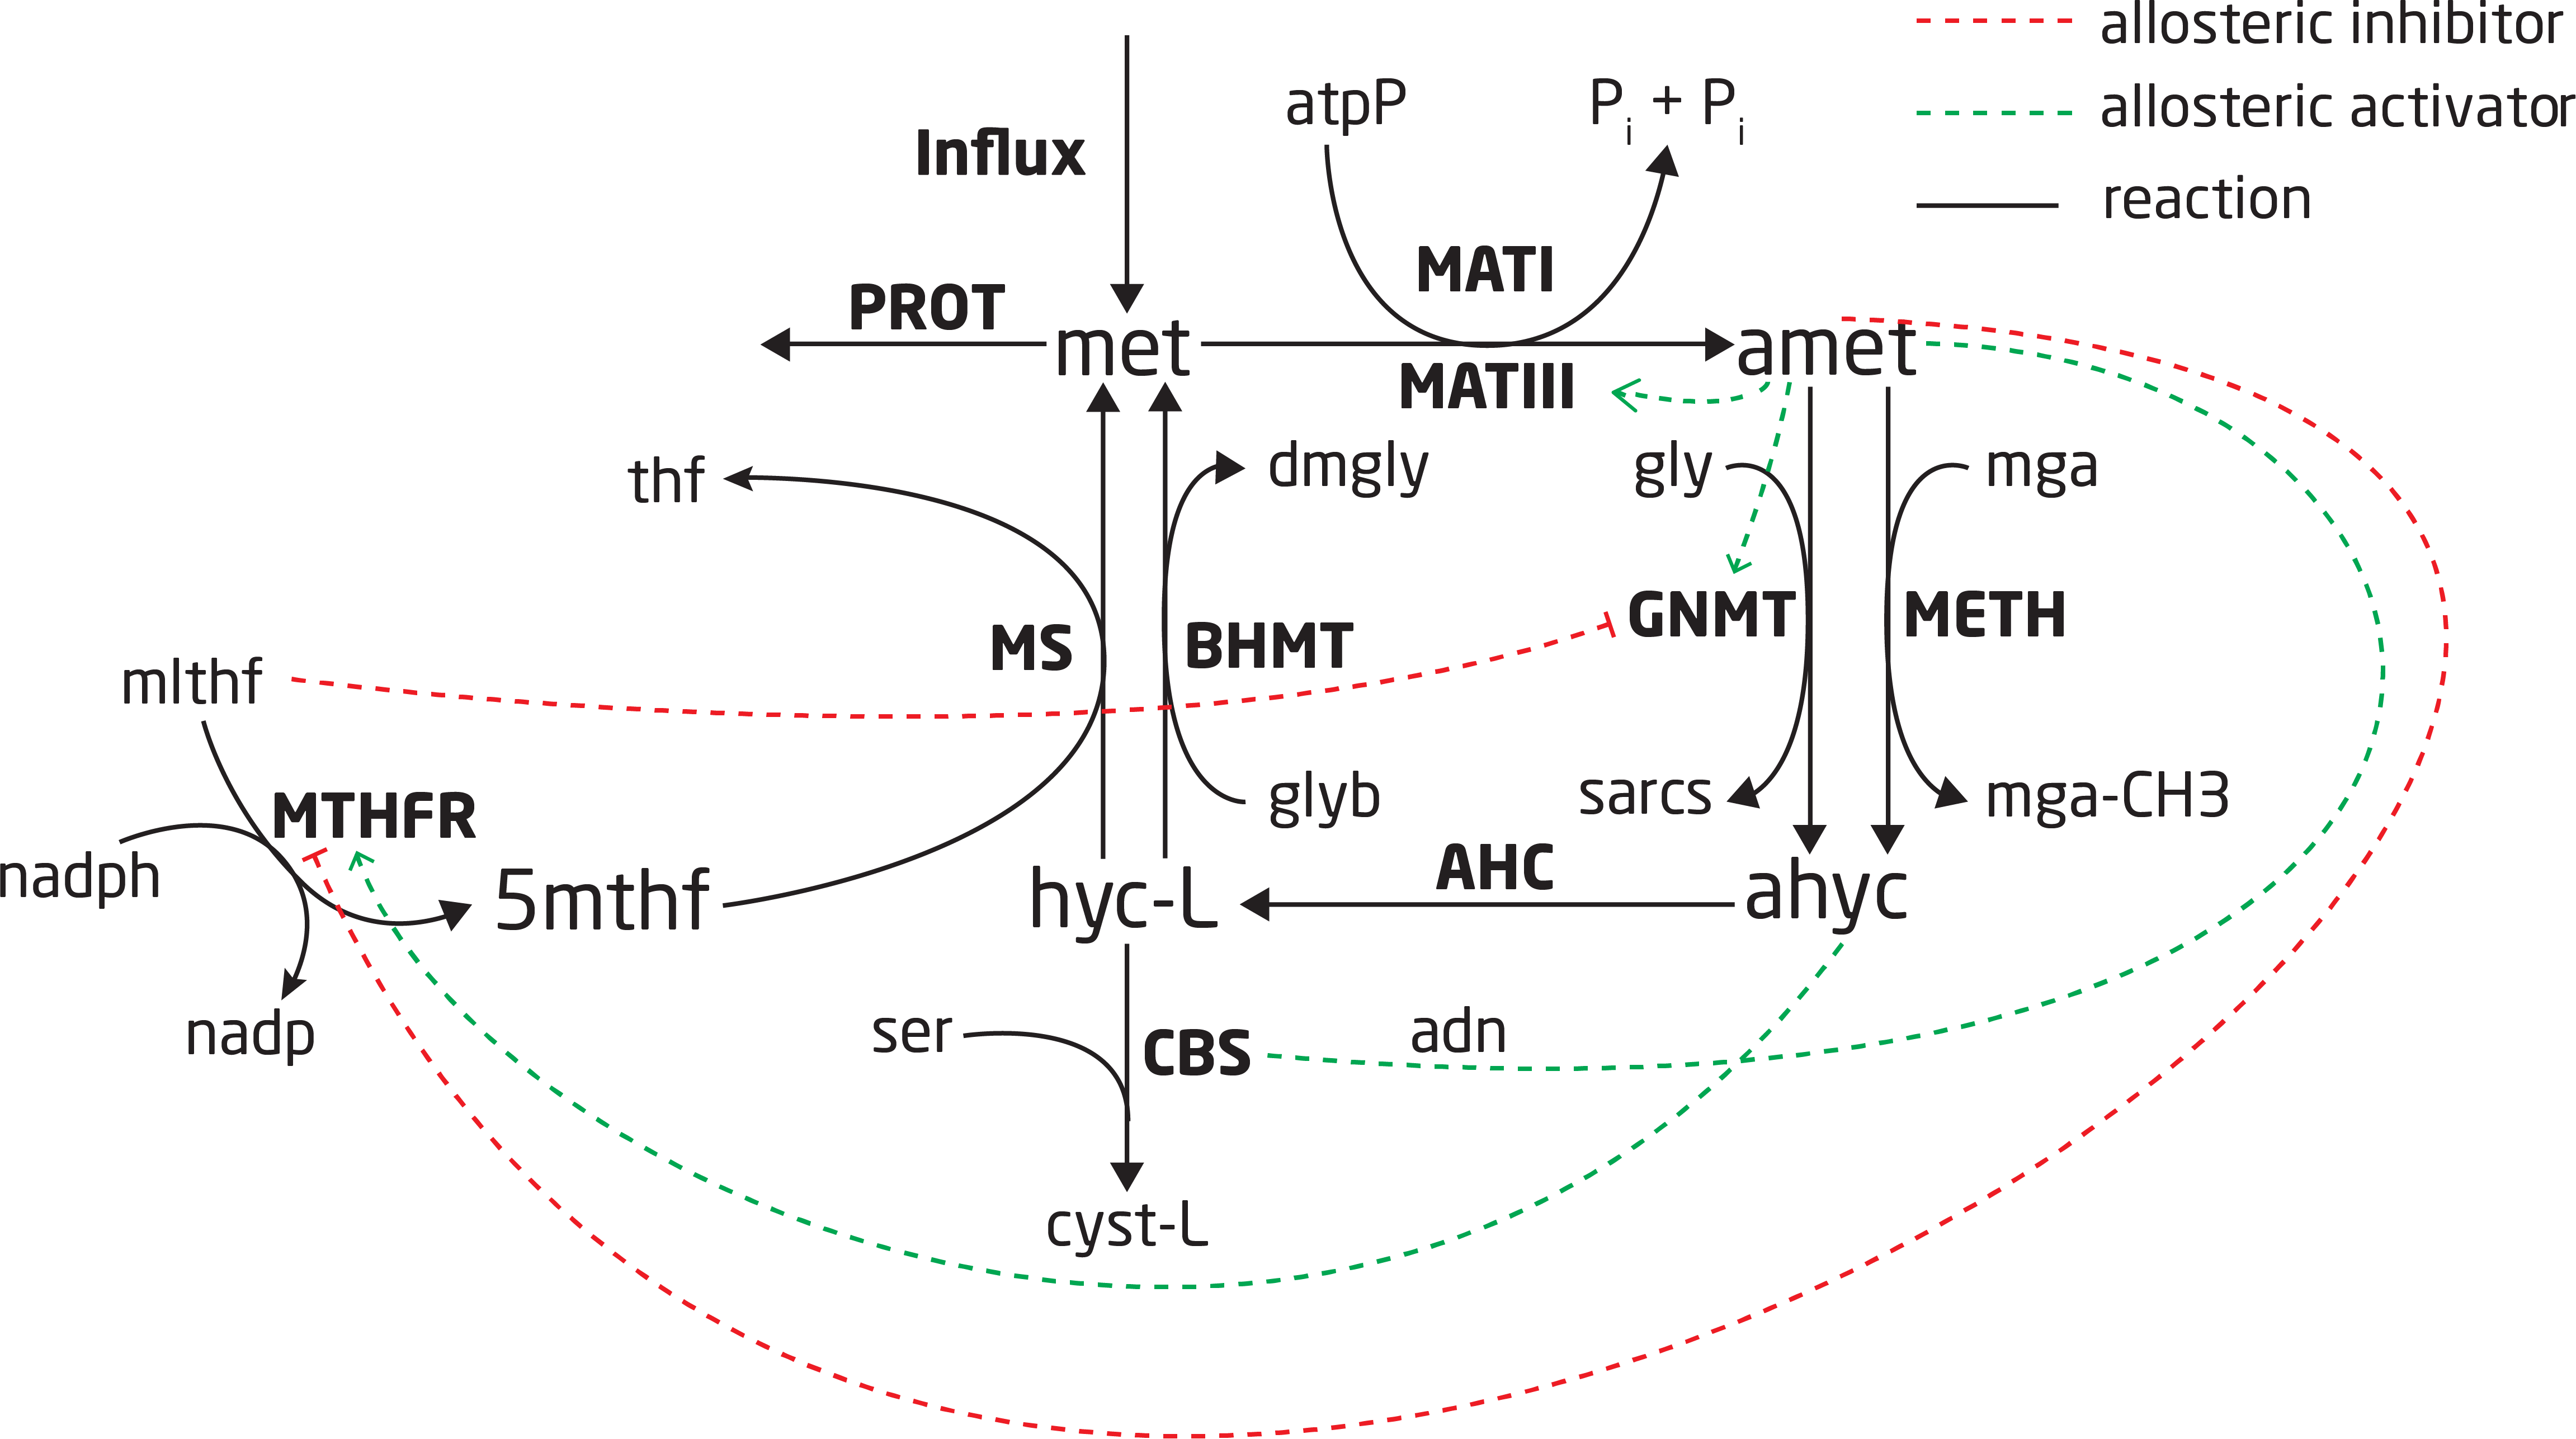
\includegraphics{./figures/methionine-reactions.png}

}

}

\end{minipage}%

\caption{\label{fig-methionine-reactions}The methionine cycle as
modelled, with the solid black lines representing the reactions, the
green lines representing allosteric interaction, and the red lines
representing allosteric inhibition. The bold fonts are the reaction
names and the regular font represents the metabolites.}

\end{figure}

\hypertarget{dataset-and-model-specification}{%
\subsection{Dataset and model
specification}\label{dataset-and-model-specification}}

The simulated dataset and underlying kinetic model that we used for our
analysis can be found at
\url{https://github.com/biosustain/Methionine_model/tree/main/data/methionine}
and is described in supplementary information section {[}REFERENCE{]}.

We constructed a kinetic model of the methionine cycle in Maud's format
using the description in \citet{korendyaseva_allosteric_2008}. The
ordinary differential equation system describing this model is shown in
Equation\,\eqref{eq-meth-ode}.

\begin{align}
\frac{d[met]}{dt} &= v_{Influx} - v_{PROT} - v_{MAT} +v_{MS} + v_{BHMT} \label{eq-meth-ode} \\
\frac{d[amet]}{dt} &= v_{MAT} - v_{GNMT} - v_{METH} \nonumber \\
\frac{d[ahyc]}{dt} &= v_{GNMT} + v_{METH} - v_{AHC} \nonumber \\
\frac{d[hyc-L]}{dt} &= v_{AHC} - v_{CBS} - v_{MS} - v_{BHMT} \nonumber \\
\frac{d[5mthf]}{dt} &= v_{MTHFR} - v_{MS} \nonumber 
\end{align}

After specifying the qualitative aspects of the kinetic model, we
selected parameter values to use as ground truth by Monte Carlo sampling
using a previous model of the methionine cycle as a starting point (see
\citet{saa_general_2015} for this model).

We used these parameters to simulate steady states in a range of
plausible experimental conditions, again using \citet{saa_general_2015}
as a starting point. These steady states were then used to generate
simulated measurements using the measurement model described below in
Section~\ref{sec-methionine-measurement-model}.

\hypertarget{sec-methionine-measurement-model}{%
\subsubsection{Measurement
model}\label{sec-methionine-measurement-model}}

Generating an artificial dataset required a specification of the true
measurement error. For enzyme and metabolite concentration measurements
we specified a standard deviation of 0.1 on natural logarithmic scale,
corresponding to approximately 10\% measurement error. For each reaction
measurement a measurement standard deviation of approximately 10\% of
the simulated value.

These measurement error specifications are somewhat optimistic
considering the many sources of variation and uncertainty affecting
quantitative proteomics, metabolomics and fluxomics analyses, but are a
reasonable first approximation to a realistic set of measurements.

For our main model run, we assumed that all metabolite and enzyme
concentrations were measured, and that there was a reaction measurement
for each of the network's elementary flux modes.

\hypertarget{trainingvalidation-split}{%
\subsubsection{Training/validation
split}\label{trainingvalidation-split}}

The training testing split was selected to achieve a large difference
between the fluxes of the training and testing dataset. The split was
determined as we are interested in showing how our model can fit to
varied conditions, and conditions closer to the training set are likely
to be predicted well without necessarily learning the system.

\hypertarget{additional-dataset-with-missing-measurements}{%
\subsubsection{Additional dataset with missing
measurements}\label{additional-dataset-with-missing-measurements}}

To gain insight into our model's robustness to missing measurements, we
also performed a model run with the same 6 experimental datasets, but
with measurements of the metabolite S-Adenosyl-L-homocysteine, or
``ahcys'' removed. Since ahcys regulates three enzymes in the methionine
cycle, including one enzyme which is also thermodynamically regulated,
we expected the removal of these measurements to yield interesting
results.

\hypertarget{maud-input-specification}{%
\subsubsection{Maud input
specification}\label{maud-input-specification}}

We constructed inputs in Maud's format for each of the analysed
datasets, based on the scenario that the true kinetic model was known
except for parameter values, which needed to be inferred from the
training data and priors. These inputs can be found at
\url{https://github.com/biosustain/Methionine_model/tree/main/data}.

The prior distributions and corresponding true parameter values used in
our case study are shown in supplementary materials section
{[}REFERENCE{]}. The first two columns show the 1\% and 99\% quantiles
of each marginal prior distribution. True parameter value are shown in
column three, and the last column shows the z-score on log scale of the
true parameter value according the marginal prior distribution. As can
be seen from the table, there are 7 parameters for which the true value
is outside the 1\%-99\% range. This is desirable, making the case study
more realistic, because extreme deviance from the prior distribution is
likely to occur in practice due to in vivo to in vitro measurement
differences.

\hypertarget{computation}{%
\subsubsection{Computation}\label{computation}}

We conducted adaptive Hamiltonian Monte Carlo sampling for the full and
missing- -data datasets, obtaining XXX post-warmup samples after XXX of
total computation time. For the Laplace approximation comparison, we
used Maud's Laplace mode. Full details as well as instructions for
reproducing our analysis can be found at XXX.

\hypertarget{findings}{%
\subsection{Findings}\label{findings}}

\hypertarget{posterior-inference}{%
\subsubsection{Posterior inference}\label{posterior-inference}}

Running standard diagnostic checks indicated that the samples we
generated were from the target posterior distribution. The improved
\(\hat{R}\) statistic
\citep{vehtariRankNormalizationFoldingLocalization2021} for every
sampled variable was within 1\% of 1, indicating appropriate mixing
within and between Markov chains. Additionally, the number of effective
samples was high, indicating that we generated enough posterior samples
to support inferences about the bulks of the distributions of the
sampled parameters. Furthermore, we observed no post warm-up divergent
transitions, indicating that the sampler was able to transform the
log-posterior distribution, avoiding any regions with excessive
curvature that might inhibit exploration via HMC.

Posterior predictive checking indicated that our model achieved a good
fit to the simulated reaction and metabolite concentration measurements,
as shown by the graphs in the top row of figure 3. Note that the fit was
good for both training and validation measurements.

Analysis of the posterior distributions for kinetic parameters indicated
that these are highly correlated. The marginal posterior distributions
for most kinetic parameters did not shrink significantly compared with
the corresponding marginal prior distributions, even though these
parameters' joint posterior distribution contained enough information to
make accurate out of sample predictions. In some cases, there were
two-dimensional correlations such as the one shown in the bottom left of
figure 3; in this case the marginal distribution of the two parameters
is roughly banana shaped. More commonly, however, two-dimensional pair
plots were insufficient to reveal the underlying correlation structure,
as seen in the bottom-right plot in figure 3. This does not mean that
the parameters were uncorrelated, but rather that the correlations
involve more than two parameters.

Overall, our results show that Maud can fit a realistic pathway-sized
dataset. This was achieved without fixing the marginal values of kinetic
parameters: the information required to make good predictions was
contained in the correlation structure of the joint posterior
distribution. This finding is consistent with previous analyses of
biological systems that found they are ``sloppy'', that is, sensitive to
parameter combinations rather than marginal parameter values, with
important combinations, scales and regions of sensitivity being
difficult to ascertain in advance
\citep{gutenkunst_2007, poirier_revising_1998}.

The question naturally arises whether the crucial high-dimensional
parameter correlations are linear or non-linear. This is relevant to the
question of model performance, as linear correlations are easier to
correct for. A linearly correlated posterior space would also be easier
to summarise. We address this question below in
Section~\ref{sec-laplace}.

This case study illustrates the type of kinetic model and dataset that
Maud can fit. The model we analysed has XXX reactions, XXX state
variables and XXX parameters. Posterior sampling with adaptive
Hamiltonian Monte Carlo generated XXX ESS/hour. Generalising from this
result, we conclude that it is feasible to use this method to fit models
in the same order of magnitude, but not, for example, genome-scale
kinetic models. To fit larger models, faster steady state solving
methods or alternative inference algorithms will be required.
Section~\ref{sec-laplace} addresses whether Laplace approximation is a
suitable candidate.

\hypertarget{sec-laplace}{%
\subsubsection{Comparison with Laplace
approximation}\label{sec-laplace}}

We found that the Laplace method was not able to produce an accurate
posterior approximation for our model and dataset.

The Laplace approximation yielded XXX samples in XXX time. The
diagnostics indicated that our algorithm was able to find the maximum a
posteriori parameter configuration, approximate the Hessian and use
these quantities to generate approximate posterior samples. The results
can be found at
\url{https://github.com/biosustain/Methionine_model/tree/main/results}.

Figure~\ref{fig-laplace} summarises the results of comparing the Laplace
approximation of our case study's posterior distribution with the true
posterior. As can be seen from the top left plot, the Laplace method
does not provide a good approximation to the true posterior
distribution, as the marginal distribution of the total log probability
density is clearly different. This was confirmed using the
Kolmogorov-Smirnov test, which is a test to differentiate two empirical
univariate distributions. The two distributions were significantly
different with a p-value indistinguishable from zero.

The difference between the Laplace approximation output and the true
posterior distribution manifests itself not only in the parameter space,
but also in the measurement space. Figure 5 frame B compares the
5\%-95\% interval for flux measurement log likelihoods in the true
posterior with the Laplace approximation; lower log likelihood values
indicate that the modelled and measured values are further away. The
graph shows that the Laplace approximation yielded significantly worse
predictions than the true posterior, even for the training data.

To further explore why this is the case we compared samples from the
true posterior and the Laplace approximation for the pairwise marginal
distributions of two Michaelis-Menten constants {[}LATEX CONSTANT{]}-
and {[}LATEX CONSTANT{]}: see the bottom right cell of figure 5. This
comparison demonstrates that the Laplace method is not able to capture
the correct relationships between parameters' distributions.

This result shows that MCMC, while slower than Laplace approximation, is
unfortunately preferable for posterior inference in this case. We expect
that this is typical of kinetic models of realistic metabolic networks
in general, so we recommend that Maud users use MCMC sampling if
possible.

Our results here also provide circumstantial evidence that the parameter
correlations in Bayesian kinetic model posteriors tend to be non-linear,
as a posterior with only linear correlations would likely be more
germane to Laplace approximation. A conclusion that we drew from this
analysis was that the results of fitting our model cannot be summarised
simply, for example by fitting a multivariate normal distribution to the
posterior draws. We therefore recommend that Maud users store the full
set of MCMC draws rather than using such an approximation. This does not
preclude the possibility that there is an alternative, more compact, way
to summarise the results of Bayesian kinetic model inference; we leave
research into this topic to future work.

\begin{figure}

\begin{minipage}[t]{\linewidth}

{\centering 

\raisebox{-\height}{

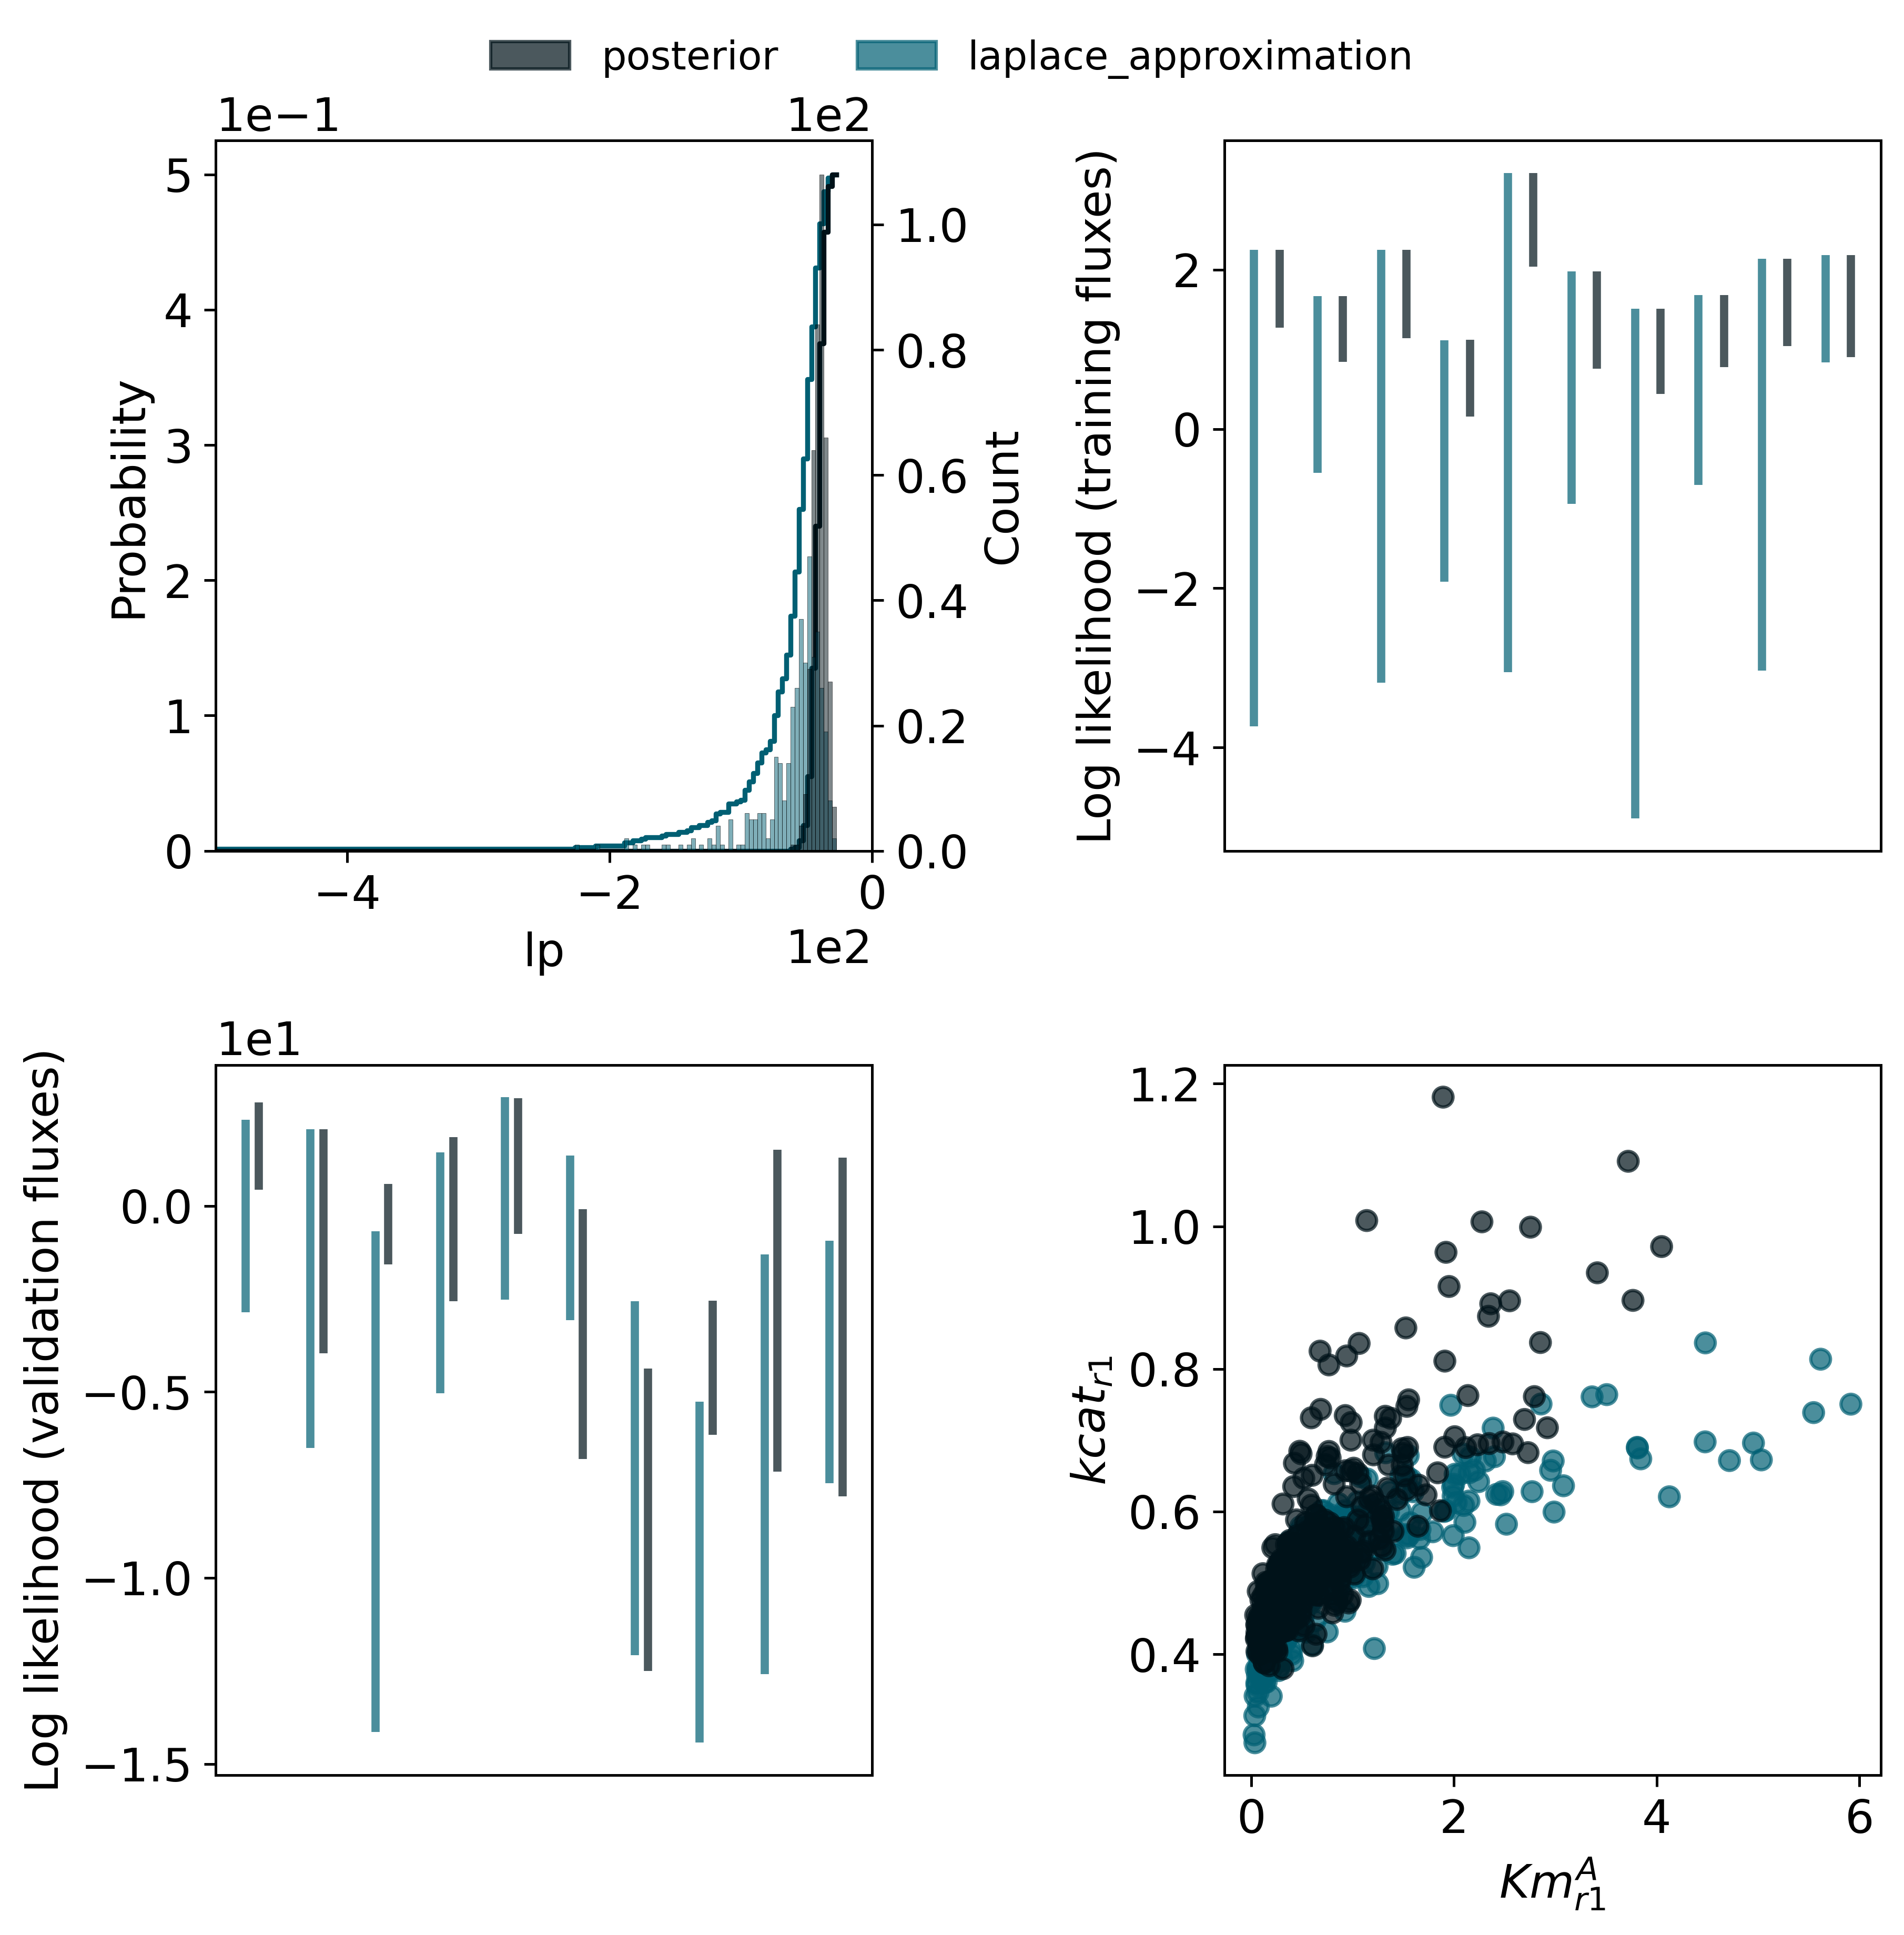
\includegraphics{./figures/laplace.png}

}

}

\end{minipage}%

\caption{\label{fig-laplace}CAPTION: FILL THIS IN!}

\end{figure}

\hypertarget{effect-of-missing-metabolite-concentration-measurements}{%
\subsubsection{Effect of missing metabolite concentration
measurements}\label{effect-of-missing-metabolite-concentration-measurements}}

Comparing model runs with and without the ahcys measurements showed that
Maud can produce sensible results even from incomplete metabolomics
data.

Figure~\ref{fig-missing} shows that, as might be expected, the model
with missing measurements did not correctly infer the missing ahcys
concentrations. Nonetheless, the remaining measured metabolites were
still well predicted, suggesting that information about the network is
still preserved despite the missing measurements. Comparison of flux
measurements in both models also indicated that removing the ahcys
measurement did not result in catastrophic model failure.

The missing measurements did affect Maud's ability to infer parameter
values correctly. The lower left plot of Figure~\ref{fig-missing} shows
that the model with full metabolomics learned the true value for the
displayed dissociation constant, despite this value being far from the
mean of the corresponding marginal prior distribution. In contrast, the
model with missing measurements stayed in the neighbourhood of the
prior.

This result is reassuring because not having access to all measurements
is a common situation in multi-omics studies. For instance, measuring
all metabolites in a pathway can be infeasible because of limitations of
mass spectrometers, availability of standards, column effects, and
compartmentalisation. However, provided that sufficient information is
available from other sources, our approach can produce sensible results
from incomplete metabolomics data.

\begin{figure}

\begin{minipage}[t]{\linewidth}

{\centering 

\raisebox{-\height}{

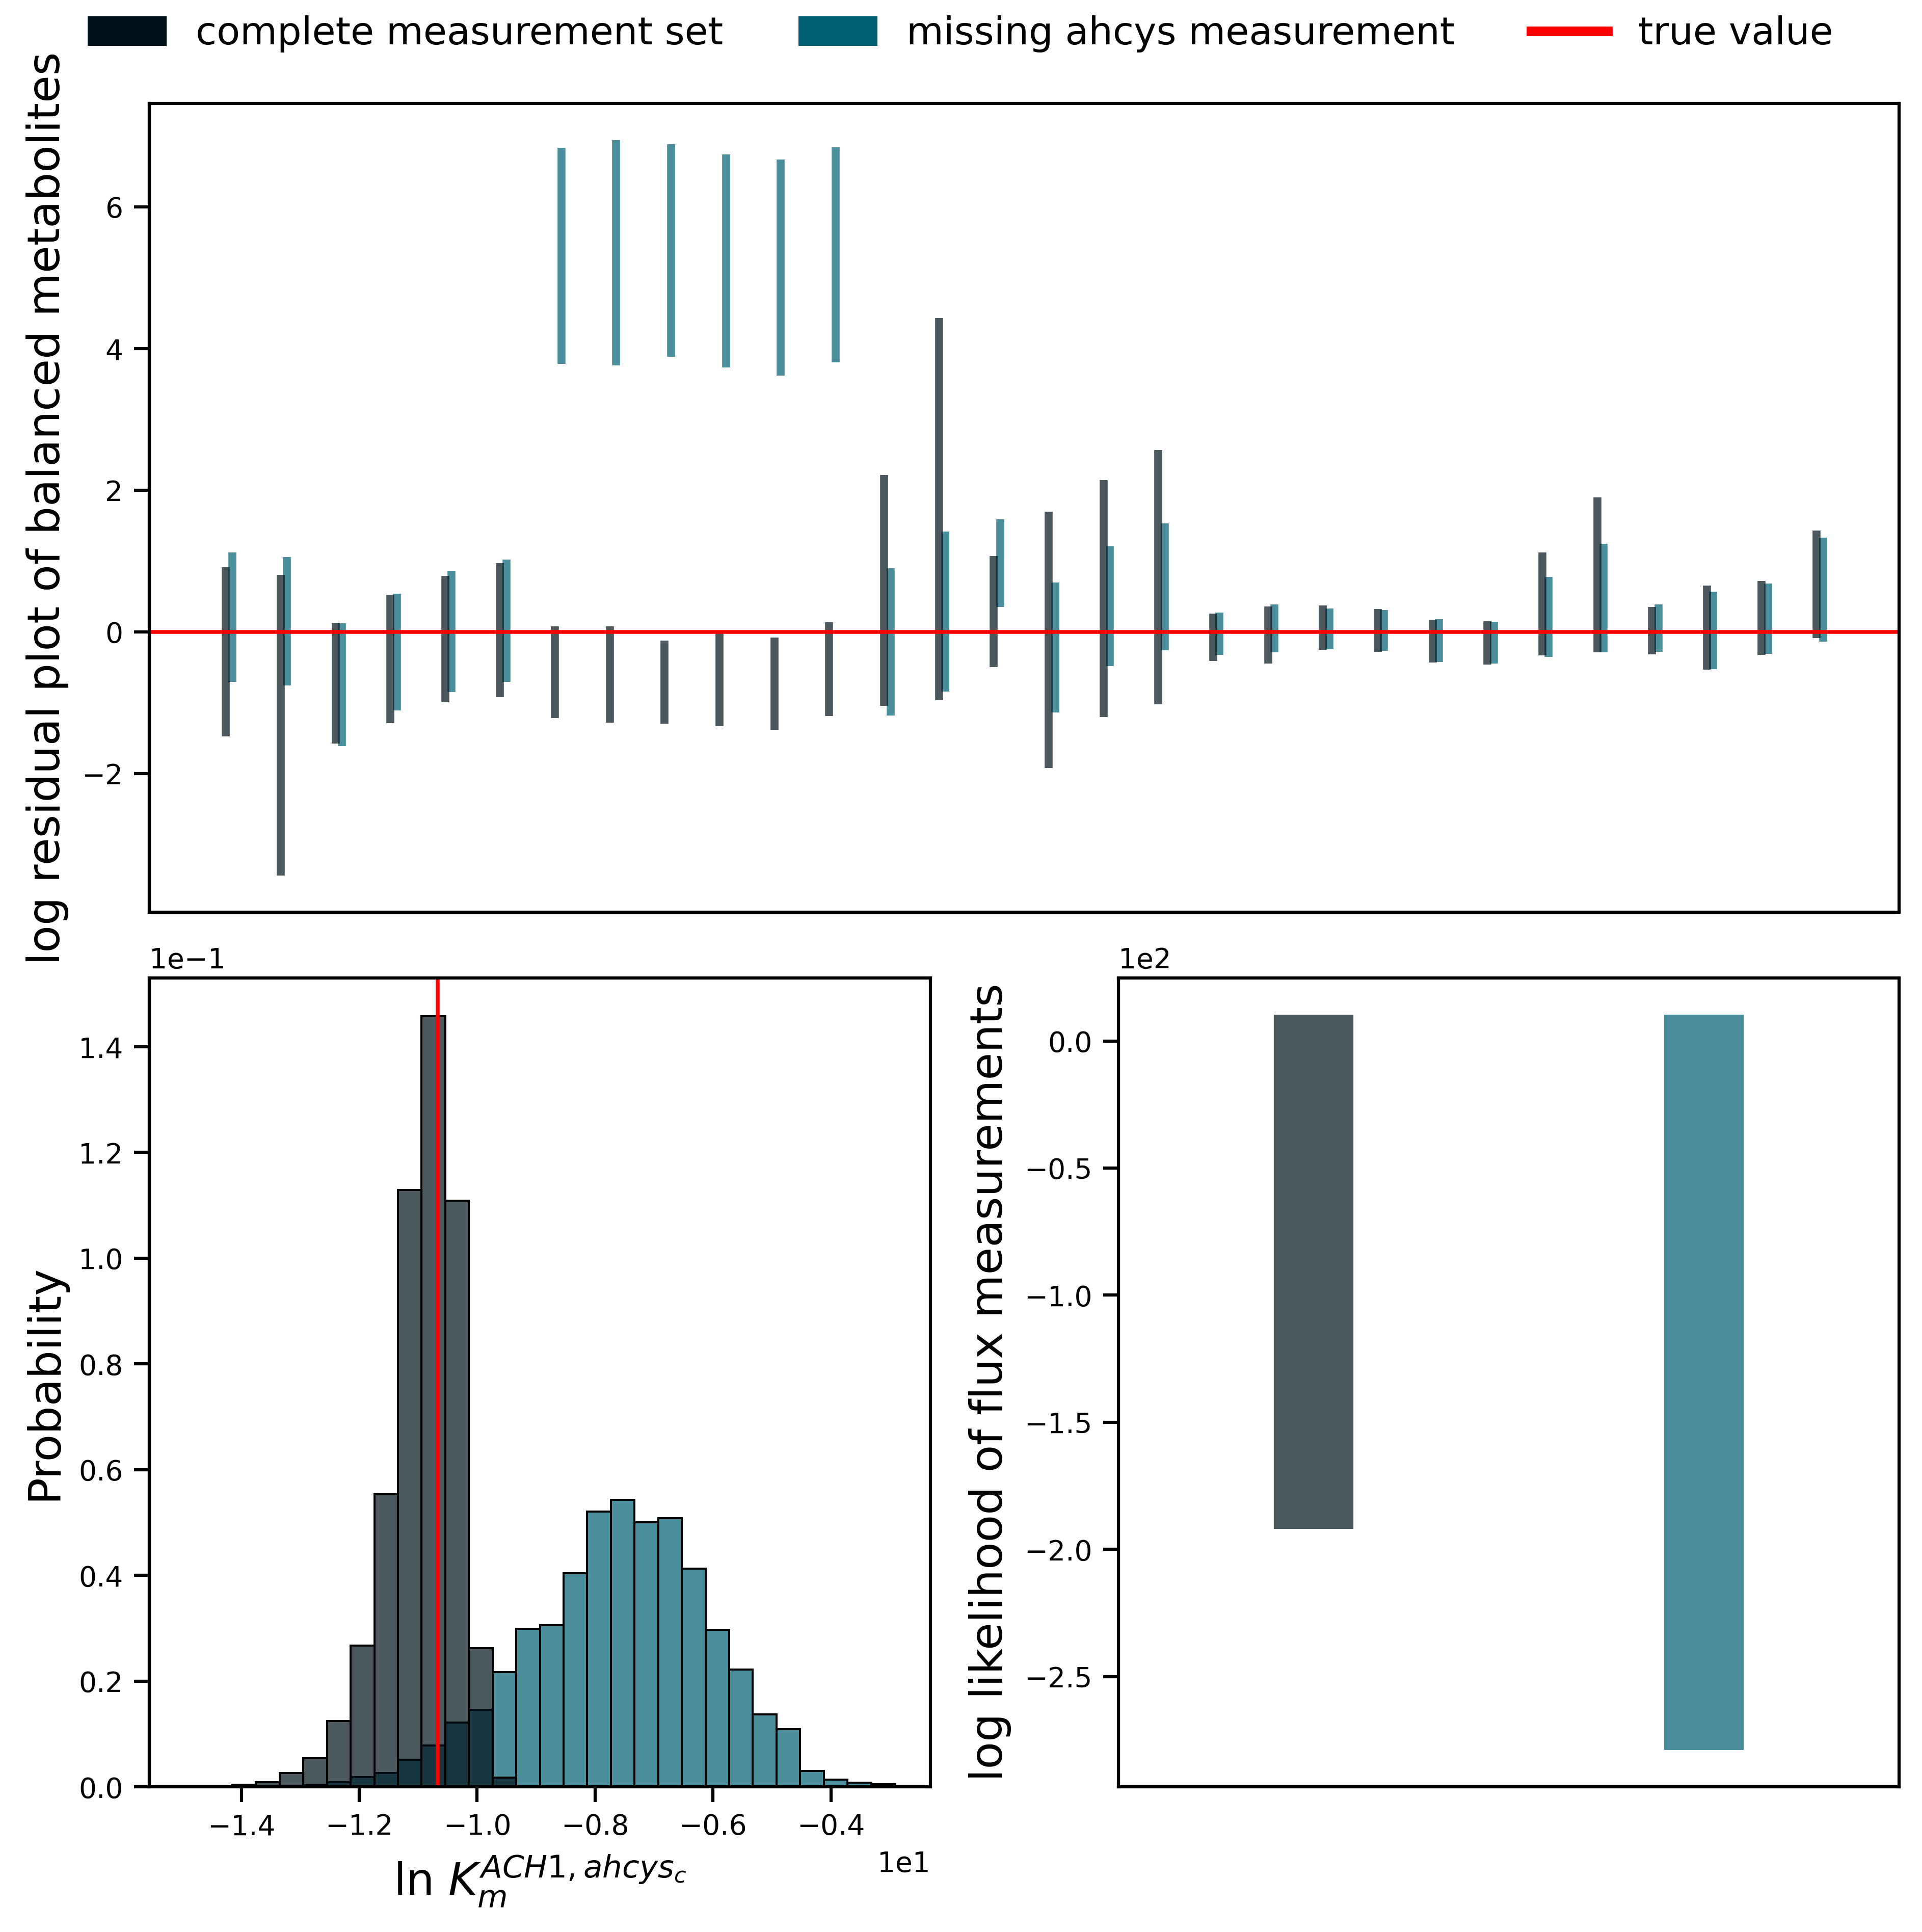
\includegraphics{./figures/missing.png}

}

}

\end{minipage}%

\caption{\label{fig-missing}Results of removing concentration
measurements for the metabolite \(ahcys_c\) from our case study dataset.
(\textbf{Top}) A comparison of metabolite concentration residuals
between the full measurement dataset (blue-green) and the missing-data
dataset (grey), displayed on natural logarithmic scale. The missing-data
model was unable to predict the withheld \(ahcys_c\) concentrations.
(\textbf{Bottom Left}) The marginal posterior distribution for the
Michaelis constant \(K_m^{AHC1,ahcys_c}\) in each model, alongside the
true parameter value used to generate both datasets. The true value is
recovered by the complete-data model but not by the missing-data model.
(\textbf{Bottom Right}) The distribution of total log-likelihood for
out-of-sample flux measurements in both models. There is a significant
overlap between the two distributions, suggesting that removing the
\(ahcys_c\) measurement did not cause catastrophic prediction failure.
However, overall the complete-data model tended to make better
predictions.}

\end{figure}

\hypertarget{application-to-regulatory-understanding}{%
\subsubsection{Application to regulatory
understanding}\label{application-to-regulatory-understanding}}

To demonstrate how Maud's output can be used to yield useful metabolic
insights we used the results of our case study to explain why the flux
of the enzyme \(GNMT\) is higher in condition 1 than in condition 2.
GNMT is an irreversible enzyme that is homotropically activated by its
substrate, competitively inhibited by its product and heterotropically
inhibited. The diverse regulation makes it the ideal test case to
elucidate regulatory changes.

Figure~\ref{fig-decomposition} shows the regulatory description of GNMT,
according to the results our main case study analysis. Each curve shows
the marginal posterior distribution of the ratio of the corresponding
regulatory component in condition 1 compared with condition 2. A
positive value indicates that the component was increased in condition 1
relative to condition 2, with 0 indicating no difference. The
probability, according to our model, of the component acting in each
direction is given by the relative area under the curve on each side of
the 0 point.

Our model correctly inferred that saturation and allosteric effects were
the main drivers of regulation between the two conditions in this case,
with the curves for each component aligning with the ground truth shown
in red.

Importantly, this form of analysis takes into account all modelled
sources of uncertainty, including uncertainty about the true values of
the flux in each condition, and propagates this uncertainty into the
final conclusion. Our result shows that Maud could be used in this
realistic case not only to provide a user with an explanation for an
observed difference in fluxes, but also a reasonable judgement as to the
explanation's robustness.

\begin{figure}

\begin{minipage}[t]{\linewidth}

{\centering 

\raisebox{-\height}{

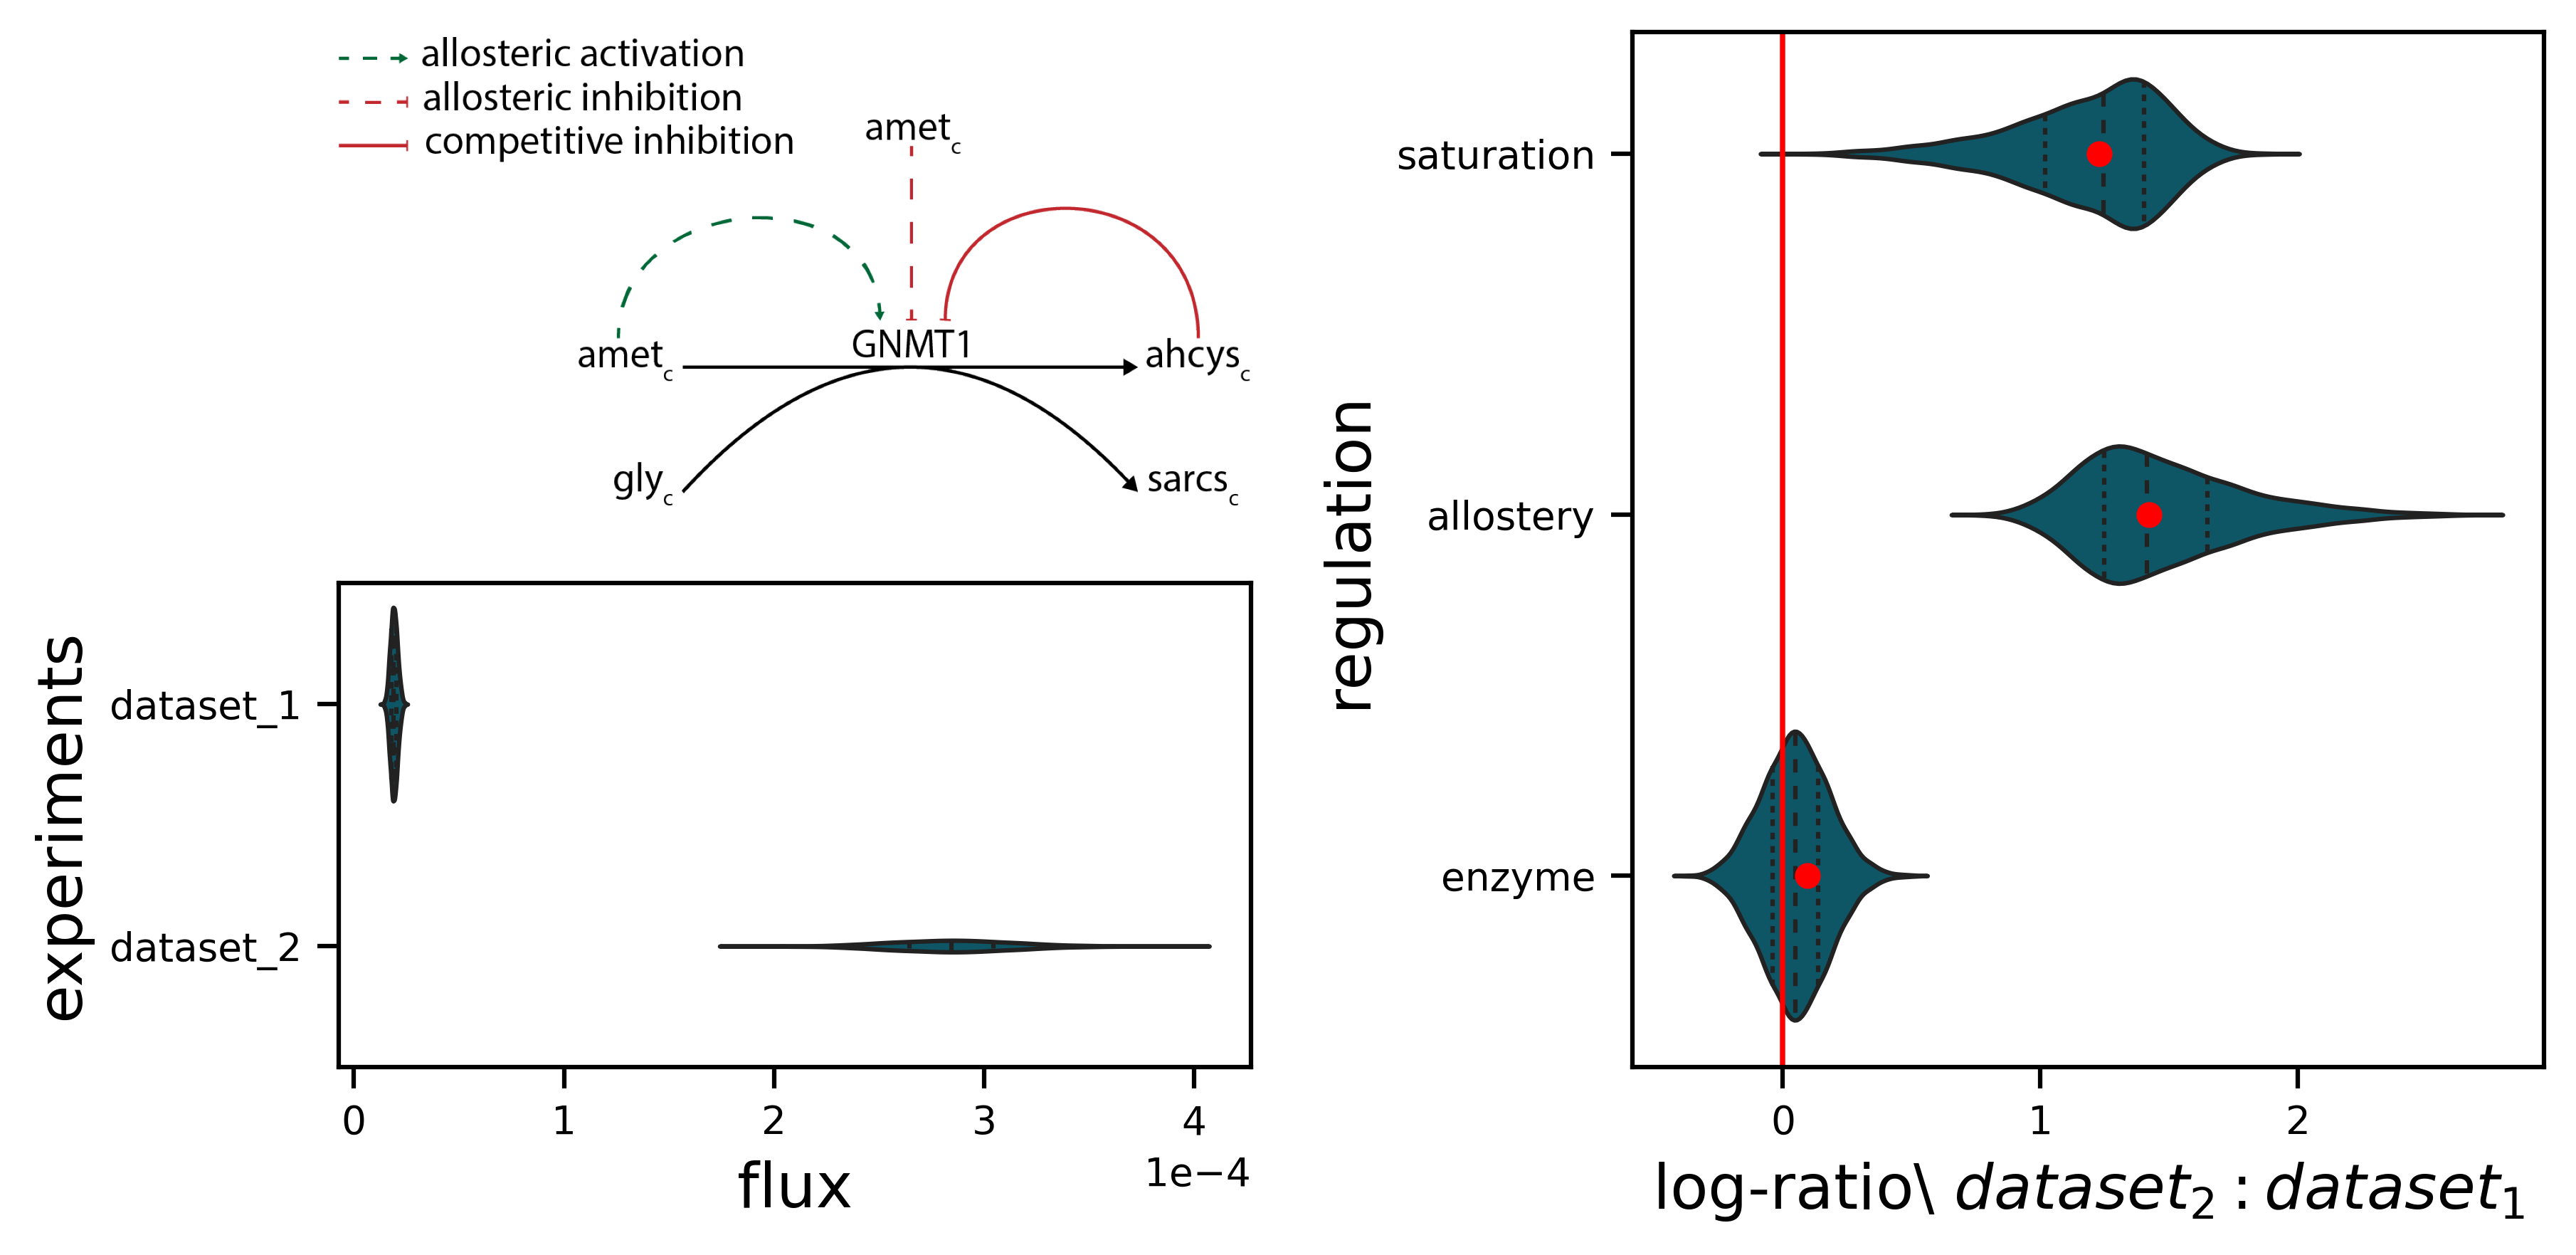
\includegraphics{./figures/decomposition.png}

}

}

\end{minipage}%

\caption{\label{fig-decomposition}Illustration of how analysing a system
with Maud can yield actionable insights about the underlying metabolic
network. (\textbf{Top Left}) A schematic of the regulatory interactions
associated with the enzyme \(GNMT1\). Dashed green lines represents
allosteric activation, dashed red lines indicate allosteric inhibition
and solid red lines represent competitive inhibition. (\textbf{Bottom
Left}) Comparison of marginal posterior distributions for \(GNMT\) flux
in conditions 1 and 2. (\textbf{Right}) Log-scale ratios of the
regulatory elements defined in equation \eqref{eq-decomposition}. Note
that the \(Reversibility\) and \(k_cat\) components are excluded: this
is because this reaction was modelled as irreversible, and \(k_{cat}\)
was modelled as constant across conditions. These plots identify why
flux in condition 2 is higher than in condition 1: the flux increase is
due to allostery and saturation with no control from enzyme
concentration changes.}

\end{figure}

\hypertarget{methods}{%
\section{Methods}\label{methods}}

Maud is a command line application implementing Bayesian inference for a
wide range of realistic kinetic models. Maud is written in Python
\citep{vanrossumPythonReferenceManual2009}, designed for use on Windows,
macOS and Linux, registered on the Python Package Index as
\texttt{maud-metabolic-models}, documented at
\url{https://maud-metabolic-models.readthedocs.io} and actively
developed and maintained at \url{https://github.com/biosustain/Maud/}.

To use Maud, a user must first collate appropriate input information,
represent it in files with Maud's required formats (see section
(REFERENCE)below). Maud's command line interface provides commands for
inference, simulation and making out-of-sample predictions. Results are
stored in files, using a structured, interoperable format.

\hypertarget{input-format}{%
\subsection{Input format}\label{input-format}}

Maud inputs are structured directories, somewhat inspired by the PEtab
format \citep{SchmiesterSch2021}. A Maud input directory must contain a
toml \citep{preston-wernertomandgedampradyunTOMLSpecification0rc2020}
file called \texttt{config.toml} which gives the input a name,
configures how Maud will be run and tells Maud where to find the other
files, allowing these to have custom names. It must also include a file
containing a kinetic model definition, a file specifying information
about parameters and a file with information experiments. The required
structure of these files is documented at \textless https://
maud-metabolic-models.readthedocs.io/en/latest/inputting.html\textgreater.
The input is validated against a Pydantic
\citep{pydanticdevelopersPydantic2022} data model which can be inspected
at \url{https://github.com/biosustain/Maud/tree/main/maud/data_model}.

We chose to implement a custom input format despite the existence of
standard formats in similar areas, including SBML
\citep{keatingSBMLLevelExtensible2020} and PEtab
\citep{SchmiesterSch2021}. This choice was partly motivated by the need
to ensure flexibility as Maud was developed, but there are also features
of SBML and PEtab that make them structurally unsuitable in this
context. Our requirements for an input format included that it be
mathematics-free, so that all mathematical details are encapsulated in
source code, and that it has a detailed, verifiable structure. These
requirements made toml more attractive than SBML: toml is easier for
humans to read and edit and can straightforwardly be validated using
tools like Pydantic. Further, an SBML representation of our desired
input would not contain differential equations. It would therefore not
be interoperable with most SBML targeting software, which typically
assumes that differential equations are available and does not know
about Maud's structure.

\hypertarget{kinetic-model}{%
\subsection{Kinetic model}\label{kinetic-model}}

Maud's kinetic model decomposes into factors as shown in equation
\eqref{eq-decomposition}.

\begin{equation}
F(C;\theta) = Enzyme\cdot k_{cat}\cdot Reversibility \cdot Saturation \cdot Allostery \label{eq-decomposition}
\end{equation}

Each of the terms on the right-hand side of \eqref{eq-decomposition} is
a function of \(C\) and \(\theta\). This idea is taken from
\citet{noor_note_2013}. The terms usefully gather physically meaningful
and conceptually distinct factors contributing to reaction fluxes.
\(Enzyme\) captures the effect of enzyme concentration, \(k_{cat}\) that
of enzyme efficiency, \(Reversibility\) quantifies thermodynamic
effects, \(Saturation\) the effect of enzyme availability and
\(Allostery\) the effect of post translational modifications.

We used the model of enzyme saturation from
\citet{liebermeister_modular_2010} and the generalised
Monod-Wyman-Changeux model of Allosteric regulation introduced in
\citep{monod_nature_1965, changeux_2013, popova_generalization_1975, popova_description_1979}
and used more recently in \citet{matosGRASPComputationalPlatform2022}.
To capture the effect on enzyme activity of coupled phosphorylation and
dephosphorylation processes we developed a new mathematical model
inspired by the generalised MWC model of allosteric regulation. Full
details of all mathematical aspects of Maud's kinetic model can be found
in supplementary material section (REFERENCE).

\hypertarget{statistical-model}{%
\subsection{Statistical model}\label{statistical-model}}

Maud represents information from measurements using generalised linear
regression models that probabilistically connect realised measurements
with true values of the measurable quantities. Information from other
sources is represented using a prior distribution over a set of latent
parameters. The parameters and the measurable quantities are connected
by a generative model encompassing Maud's kinetic model as well as the
steady state equation \eqref{eq-3}. Together, the measurement model,
prior model and generative model determine a joint probability function
that assigns a probability density to any possible combination of
measurements and parameters.

Below we describe the prior and measurement models, as the generative
model has already been discussed above.

\hypertarget{prior-model}{%
\subsubsection{Prior model}\label{prior-model}}

Maud's prior model includes unknown parameters corresponding to
quantities in the kinetic model that are assumed to be unknown, other
than steady state metabolite concentrations and fluxes, which are
derived from the values of other parameters by solving the steady state
problem. See table (REFERENCE) in this paper's supplementary materials
for a description of all these parameters and their dimensions. Note
that some quantities in Maud's kinetic model are not treated as
parameters: for example, temperatures, compartment volumes and the
formation energy of water. Maud treats these quantities as if they were
known precisely: they can be configured by the user or default values
can be used. Although in practice there can be considerable uncertainty
regarding these quantities, we chose to disregard this uncertainty in
the interest of simplicity.

Except for metabolites' standard condition Gibbs energy changes of
formation, Maud uses independent normal prior distributions for
parameters that can in principle be both negative and positive. For
parameters that are constrained to be positive, Maud uses independent
log-normal distributions. Formation energy parameters have a
multivariate normal prior distribution. Location, scale and covariance
parameters for all these prior distributions can be selected freely by
the user.

\hypertarget{measurement-model}{%
\subsubsection{Measurement model}\label{measurement-model}}

Maud's measurement model considers three types of measurement:
metabolite concentration measurements, enzyme concentration measurements
and flux measurements, represented by vectors \(𝑦^{𝑐𝑜𝑛𝑐}\) \(𝑦^{𝑒𝑛𝑧}\)
and \(𝑦^{𝑓𝑙𝑢𝑥}\) respectively.

All measurements are specific to an experimental condition; that is, a
case where the true state of the network, including knockouts, boundary
conditions and state variables as well as kinetic and thermodynamic
parameters, can safely be assumed to be the same. Maud's statistical
model allows for arbitrarily many experimental conditions, and for any
measurable quantity to be measured any number of times in any condition.

Metabolite and enzyme measurements are intended to represent the results
of quantitative metabolomics and proteomics experiments. The likelihood
functions for such measurements are shown in equations
Equation\,\eqref{eq-yconc} and Equation\,\eqref{eq-yenz}.

\begin{align}
y_i^{conc} &\sim LN(\ln{\hat{y}_i^{conc}}, \sigma_i^{conc})\label{eq-yconc} \\
y_i^{enz} &\sim LN(\ln{\hat{y}_i^{enz}}, \sigma_i^{enz})\label{eq-yenz}
\end{align}

Both equations are log-normal generalised linear models with a standard
link function (the natural logarithm \(\ln\)) and known standard
deviation \(\sigma_{𝑐𝑜𝑛𝑐}\). The use of this measurement model is
motivated by the consideration that concentrations are constrained to be
non-negative, so the measurement model should avoid assigning positive
probability mass to negative metabolite concentration values. In
addition, we expect the precision of most metabolomics and proteomics
experiments to be roughly proportional to the value of the true measured
quantity, which supports a measurement model with constant coefficient
of variation. The measurement standard deviations \(\sigma_{𝑐𝑜𝑛𝑐}\) and
\(\sigma_{𝑒𝑛𝑧}\) are assumed to be known exactly for simplicity;
plausible values can be elicited by considering the likely coefficient
of variation of the measuring apparatus.

Flux measurements, representing the results of quantitative fluxomics
analyses, are modelled using a likelihood function from a standard
linear regression model, as shown in equation\,\eqref{eq-yflux}. Flux
measurements can be obtained from the results of isotope labelling
experiments using metabolic flux analysis, for example as described in
(Young 2014). When entering flux measurements, it is important only to
specify measurements for a network's free fluxes, as the values of some
steady state fluxes in a metabolic network are constrained by others,
with the result that dependent fluxes cannot typically be measured
separately. If measurements of multiple dependent fluxes are entered,
information will inappropriately be double counted.

\begin{equation}
y_i^{flux} \sim LN(\ln{\hat{y}_i^{flux}}, \sigma_i^{flux})\label{eq-yflux}
\end{equation}

Our measurement model improves on analyses of metabolomics and
proteomics data that assume a regression model with normally distributed
errors, whether explicitly using a standard linear model or implicitly
using ordinary least squares fitting. This assumption is undesirable
because it implies that the measured quantity could in principle be
negative, and assumes an additive underlying random process, whereas
multiplicative processes tend to better describe real concentration
data.

The use of independent measurement models for metabolite, enzyme and
flux measurements carries an implicit assumption that there are no
systematic correlations in the measurement errors. This choice was
motivated by simplicity - it would be better to use a model with
potentially correlated measurements. Similarly, it would be preferable
to include measurement errors as model parameters, thereby avoiding
possible bias due to incorrect assessments of measurement accuracy.
However, we chose to use a simpler measurement model to avoid the
complexity and potential fitting issues that these changes would entail.

Finally, the reader may wonder why Maud uses a linear regression model
for reaction flux measurements even though this creates the potential
for erroneous double counting and requires non-trivial upstream
modelling, as intracellular fluxes typically cannot be measured
directly. Instead, fluxes are typically inferred from isotope labelling
experiments using metabolic flux analysis: see
\citet{daiUnderstandingMetabolismFlux2017} for more about this method.
Ideally Maud's measurement model for fluxes would extend from fluxes to
the results of potential labelling experiments, thereby removing the
need for upstream analysis and avoiding any double counting. This option
has not yet been pursued, again for the sake of simplicity.

\hypertarget{implementation}{%
\subsection{Implementation}\label{implementation}}

Maud uses the Python library click
\citep{clickdevelopersClickPythonComposable2022} to implement a command
line interface. The command line interface loads input files as Python
dictionaries, which are parsed using the Python library \texttt{toml}
\citep{pearsonTomlPythonLibrary2020} and then validated and converted
into structured \texttt{MaudInput} objects using Pydantic
\citep{pydanticdevelopersPydantic2022}. Maud's statistical model is
implemented in the probabilistic programming language Stan
\citep{carpenterStanProbabilisticProgramming2017} and accessed using the
interface cmdstanpy \citep{standevelopmentteamCmdStanPy2022}. For
posterior sampling, Maud uses the \texttt{MaudInput} to create a Stan
input json file and obtain configuration information for cmdstanpy,
which it uses to (if necessary) generate a model executable file and
then trigger posterior sampling using adaptive Hamiltonian Monte Carlo.
When sampling is complete, Maud converts to the output into the standard
format \texttt{InferenceData} using the Python library arviz
\citep{kumarArviZUnifiedLibrary2019} and saves it as a json file, along
with some information for debugging.

Two details of Maud's implementation are important to highlight: the
method of posterior sampling and how Maud solves the steady state
problem \eqref{eq-3}.

\hypertarget{posterior-sampling}{%
\subsubsection{Posterior sampling}\label{posterior-sampling}}

Although integrals of the joint probability model for kinetic models are
typically analytically intractable, they can be approximated numerically
using Markov Chain Monte Carlo (MCMC) and other methods. Maud uses MCMC
primarily because there exist many methods for verifying that MCMC
samples really do approximate the target probability distribution: see
\citet{vehtariRankNormalizationFoldingLocalization2021} and
\citet{taltsValidatingBayesianInference2018} for discussion of this
point. In addition, there are several examples of successful Bayesian
kinetic modelling projects using MCMC including
\citet{st.johnBayesianInferenceMetabolic2018} and
\citet{xingModelingKineticsLargescale2010}.

\hypertarget{solving-the-steady-state-problem}{%
\subsubsection{Solving the steady state
problem}\label{solving-the-steady-state-problem}}

In order to implement adaptive Hamiltonian Monte Carlo, Maud must
repeatedly solve the steady state problem \eqref{eq-3} and find its
gradients with respect to all parameters. To achieve this, Maud uses a
hybrid method involving two numerical solvers from the SUNDIALS suite
\citep{serbanCVODESSensitivityEnabledODE2005}: CVODES and IDAS. These
solvers are accessed via their interface from Stan. The hybrid method
follows that proposed by \citet{margossianComputingSteadyStates2018},
and involves numerically evolving the ODE system for a short period of
time, then using the difference between the evolved and starting
concentrations as the target for a numerical algebra solver.

\hypertarget{acknowledgements}{%
\section{Acknowledgements}\label{acknowledgements}}

\hypertarget{references}{%
\section{References}\label{references}}

\renewcommand{\bibsection}{}
\bibliography{bibliography.bib}




\end{document}
